\documentclass[journal]{IEEEtran}

\ifCLASSINFOpdf
\else
   \usepackage[dvips]{graphicx}
\fi
\usepackage{url}

\hyphenation{op-tical net-works semi-conduc-tor}

\usepackage{graphicx}
\usepackage{hyperref}
\hypersetup{colorlinks=true, linkcolor=blue, urlcolor=cyan}
\usepackage{bm}
\usepackage{mathtools}
\newcommand{\myMatrix}[1]{\bm{\mathit{#1}}}

% Macro to get code font
\def\code#1{\texttt{#1}}


\begin{document}

\title{AMATH 582 Homework 3: Principal Component Analysis}

\author{Eric A. Silk
\thanks{Eric Silk is a Masters Student in Applied Mathematics at the University of Washington,
		and a Research Engineer for Schweitzer Engineering Laboratories, Pullman, WA 99163 (email: esilk16@uw.edu, eric.silk@ericsilk.com)}
}

\markboth{Homework Submission for AMATH 582: Computational Methods for Data Analysis, February 2020}
{Shell \MakeLowercase{\textit{et al.}}: Bare Demo of IEEEtran.cls for IEEE Journals}
\maketitle

\begin{abstract}
Principal Component Analysis (PCA) is a highly useful technique for exploratory data analysis which decomposes a series of observations along axes of the most variance, which then allows for discarding of the less important variables to project into a lower dimensional subspace. This report explores its use in tracking the motion of paint can.
\end{abstract}

\begin{IEEEkeywords}
Singular Value Decomposition, Principal Component Analysis, Object Tracking, OpenCV
\end{IEEEkeywords}


\IEEEpeerreviewmaketitle


\section{Introduction}
\IEEEPARstart{P}{r}incipal Component analysis is a technique used to determine the best method of
representing data in a lower dimensional subspace. It works by using an orthogonal transformation
to convert data which may be correlated into a series of vectors which are uncorrelated. In a 
ense, it can produce the ``best" basis by which to represent a set of data.

In order to explore this method, we will perform PCA upon the motion of a flashlight attached to a
paintcan, moving in a variety of patterns (simple oscillation, oscillation and pendulum motion,
oscillation, pendulum, and spinning), measured by cameras in three arbitrary positions and 
orientations.

\section{Theoretical Background}
\subsection{PCA}
 The technique of Principal Component Analysis works by computing the eigenvalues and eigenvectors
 of the covariance matrix of the data matrix $ \myMatrix{X} $, which is defined as
 $ \myMatrix{X}\myMatrix{X}^{T} $. Calculating this directly can be numerically problematic --
 instead, the Singular Value Decomposition can be used.

 \subsection{SVD}
For full details of the computation, see Dr. Kutz's Book, ``Data-Driven Modeling and Scientific
Computation."

In short, however, SVD of a data matrix produces three matrices:
\begin{equation}
    svd(\myMatrix{X})=\myMatrix{U} \myMatrix{\Sigma} \myMatrix{V}^{*} 
\end{equation}

These resulting matrices can be interpreted within the context of this exercise as follows:
\begin{enumerate}
    \item $\myMatrix{U}$: Each column contains the direction of the PCA modes.
    \item $\myMatrix{\Sigma}$: Singular values on the diagonal, representing the energy of each mode.
    \item $\myMatrix{V}$: Each column represents the displacement in time along a mode
\end{enumerate}

In an example provided by Kelsey Maass on Piazza, the meaning of the $\myMatrix{U}$ and
$\myMatrix{V}$ matrix are swapped. This is becasue the data matrix $\myMatrix{X}$ arranges the
observations as columns, rather than rows, which is opposite the convention used in Dr. Kutz's
book.

\subsection{Properties}

One of the most important properties of this technique is a relative independence from the bases
used in the initial observation of the data. For instance, in this homework, we are given three
perspectives that are clearly non-orthogonal. Because of our a priori knowledge of the system, we
could conceivably transform the data to force a better perspective. In many cases, this isn't
possible. Use of SVD/PCA will allow us to do this more generally. More importantly, PCA will tell
us which of the modes are most critical in describing the phenomena. This can be used in a number
of ways:

\begin{enumerate}
	\item Data Exploration, to find the "important" modes to investigate further
	\item Feature Engineering, to feed a more limited subset of data to a machine learning algorithm
	\item Visualization, to project a high dimension dataset into a visualizable subspace
	\item Lossy compression, by discarding the lower energy modes
\end{enumerate}

\section{Algorithm Implementation and Development}

\subsection{Object Tracking}

Object tracking proved to be a large portion of the project. In the end, OpenCV with Python
bindings was used to identify and track an object of interest.

\subsubsection{Thresholding}
In order to facilitate object isolation, and given that the paint can had a lit flashlight on top
of it, a simple thresholding of the grayscale image was optionally applied. Specifically, a
``to zero" threshold was used. This works by identifying regions of luminance less than the
threshold and setting them to zero. Comparatively, a binary threshold sets areas below the
threshold to zero and areas above to the maximum luminance. 

\subsubsection{Bounding Box Selection}
The first frame of the video is held on screen until the user draws a bounding box around the
object of interest and presses either the space or enter key. This works quite well in most cases,
except in instances in which the primary point of interest (the lit side of the flashlight) is not
immediately visible.

\subsubsection{Tracking}
Once the bounding box is selected, a tracker provided by OpenCV was used. Specifically, the
\code{CSRT} tracker, or ``Discriminative Filter with Channel and Spatial Reliability" tracker (I'm
unsure how the acronym matches, but alas). This was the best choice in a rather non-rigorous series
of tests, and is touted as a fairly accurate method (albeit more computationally expensive than
some other objects).

One major issue that was noted was, in the event of object occlusion or other loss of tracking,
there was very poor recovery behavior. If this was to be in production, some other method of object
detection would be required, or manual re-selection of the object upon failure.

\subsubsection{Saving of Data}
Upon conversion completion, any failures to track would be recorded as \code{NaN}, and the total
number of these were reported. If the user felt they were acceptable, the data was then saved as
\code{.npy} file for easy import.

\subsection{SVD/PCA}

\subsubsection{SVD}
Fortunately, per instructor permission, the SVD itself was able to be done using a pre-built
implementation. Specifically, \code{numpy.linalg.svd}, which wraps \code{LAPACK}'s \code{\_gesdd}
routine, allowing for high numerical precision and speed.

The observation vectors were stacked before calculating the SVD, truncating to the length of the
shortest for a given case.

\subsubsection{Plotting and Exploration}
Following the example set in Dr. Kutz's book, a series of four plots were made for each case:
\begin{enumerate}
	\item Modal Energy
	\item Modal Energy, on SemiLog axes
	\item Modal behavior of the 2 most significant modes
	\item Temporal behavior of the 2 most significant modes
\end{enumerate}

Additionally, reconstruction of the SVD with only $N$ modes was performed to observe the effects of
discarding lower energy modes.


\section{Computational Results}

\subsection{Kutz Plots}
The results as ``Kutz Plots" (described in ``Plotting and Exploration") for each of the cases can 
be seen in Figures \ref{kutz1}, \ref{kutz2}, \ref{kutz3}, and \ref{kutz4}.

\begin{figure}
	\centerline{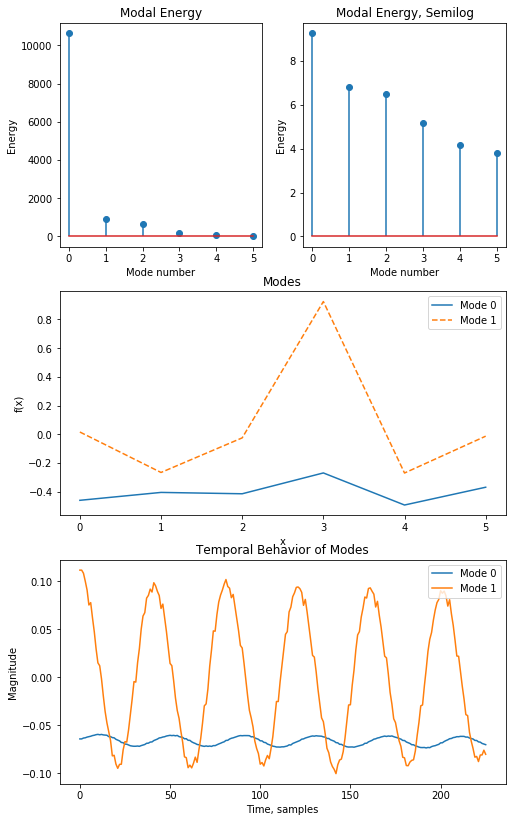
\includegraphics[width=\columnwidth]{kutz1.png}}
	\caption{Kutz Plot, Case 1}
	\label{kutz1}
\end{figure}

The first results (Fig. \ref{kutz1}) appear fairly straightforward. We know that only one major mode exists
in the data -- strong motion in the Z direction; however, PCA indicates there are two modes. Why
is this occuring? Little to no effort was made to synchronize the videos during image tracking. As
such, looking at the temporal behaviors of each mode, we can observe what appears to be a ``lag" or
``phase shift". I believe this is due to the same phenomena (the oscillation) being observed at a
slightly delayed time.

It is also worth noting that the modal directions themselves are comprised primarily of one or two
directions. This corresponds to the known orientation of the cameras and the motion relative
to that.

If the videos were perfectly synchronized, through the use of a ``clapper" or similar, I'm
certain these two modes would collapse into one strongly dominant mode. Alternatively, if time
permitted, manual re-alignment in post could achieve a similar goal.

\begin{figure}
    \centerline{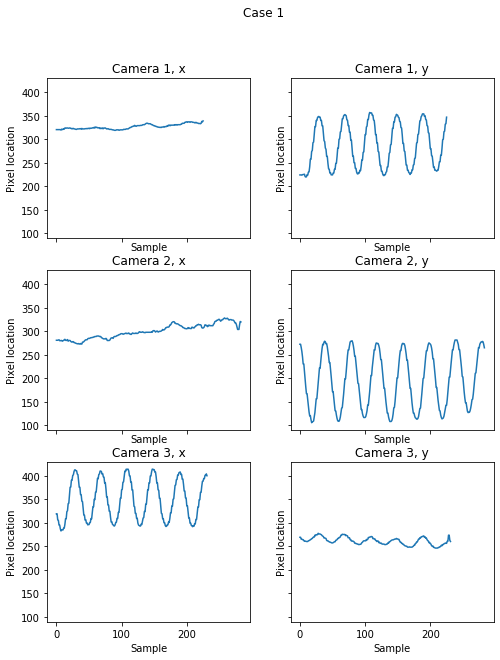
\includegraphics[width=\columnwidth]{case1.png}}
    \caption{X and Y positions of the object in each camera, Case 1}
    \label{case1}
\end{figure}

This is supported by inspecting Fig. \ref{case1} and noting that while camera 1's y location and
camera 3's x location both start in a ``trough" whereas camera 2's y location begins at a ``peak",
suggesting out of phase behavior.

\begin{figure}
	\centerline{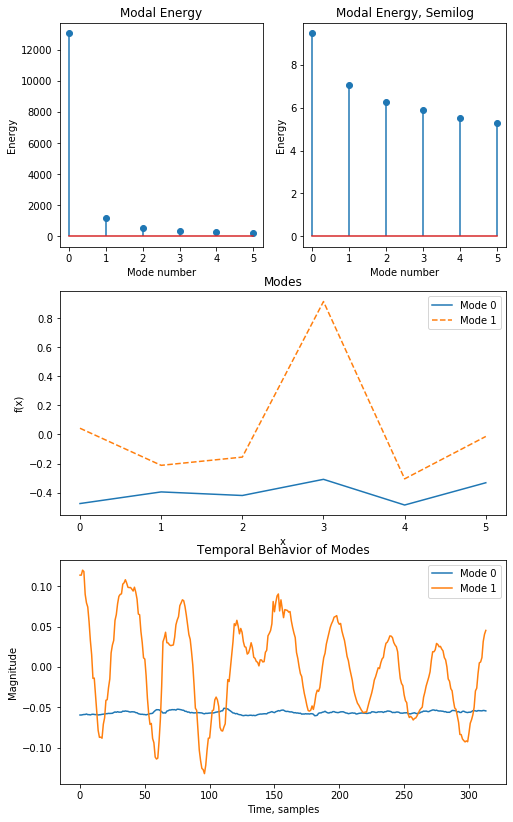
\includegraphics[width=\columnwidth]{kutz2.png}}
	\caption{Kutz Plot, Case 2}
	\label{kutz2}
\end{figure}

Based upon this, the results in the shaken camera case (Fig. \ref{kutz2}) are reasonable. The
introduction of noise raises the modal energy floor. Instead of the ideal of one clearly dominant
mode (or even 2, as explained in case 1), secondary modes also become candidates. Additionally,
the modal directions become more mixed, with contributions from more modes. This makes sense, as
the introduction of shake looks like travel along other dimensions.

\begin{figure}
	\centerline{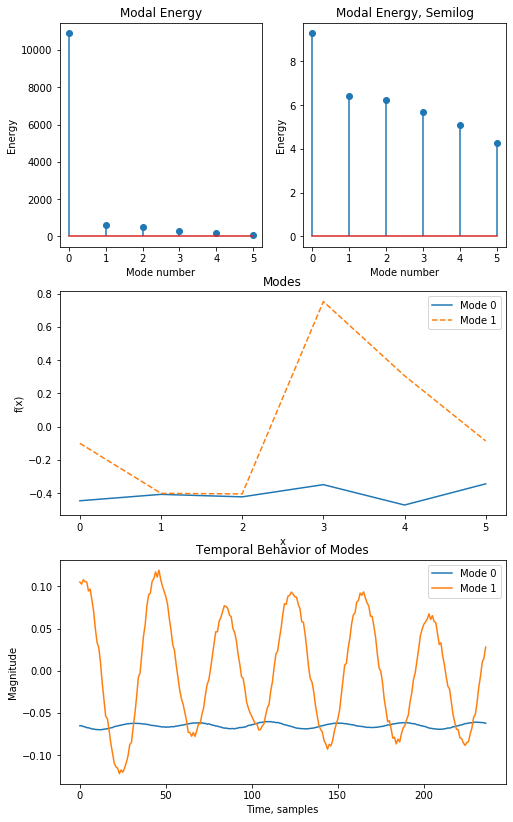
\includegraphics[width=\columnwidth]{kutz3.png}}
	\caption{Kutz Plot, Case 3}
	\label{kutz3}
\end{figure}

Introducing another dimension of motion in the form of pendulum-like oscillations, along with
the previously stated issues of synchronization, produce results that aren't unexpected. Ideally,
two modes would dominate in Fig. \ref{kutz3}, but instead 3 seem to be of significance. Again,
I believe this can be explained by comparing the relative peaks and valleys of the X and Y
coordinates in each of the camera's recordings (Fig. \ref{case3}).

\begin{figure}
    \centerline{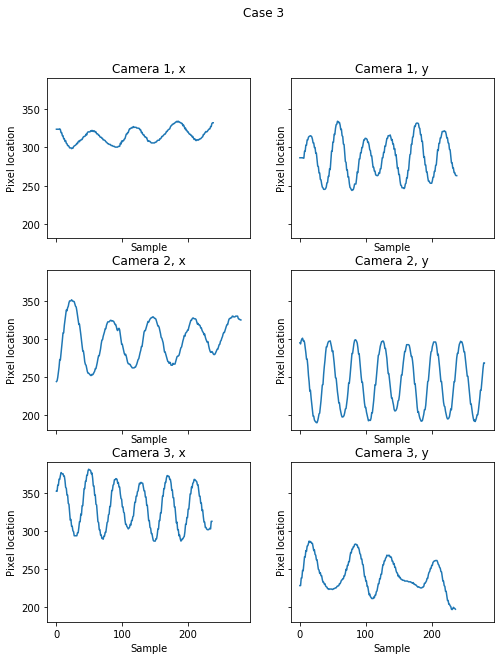
\includegraphics[width=\columnwidth]{case3.png}}
    \caption{X and Y positions of the object in each camera, Case 3}
    \label{case3}
\end{figure}

Finally, case 4 introduces rotation. Since this is being mapped to rectangular coordinates,
I would expect to see an additional mode corresponding to the "depth" direction. Looking at the
resulting modal directions and temporal behavior of each component, this seems correct. The added
modal directions of each mode are largely independent of each other. The first two temporal trends
appear to be oscillatory, corresponding to the spring and the pendulum action, while the third
shows a ``flattening" at several points (most notably in the span between samples 100 and 150),
likely corresponding to the paint can's rotation reversing.

\begin{figure}
	\centerline{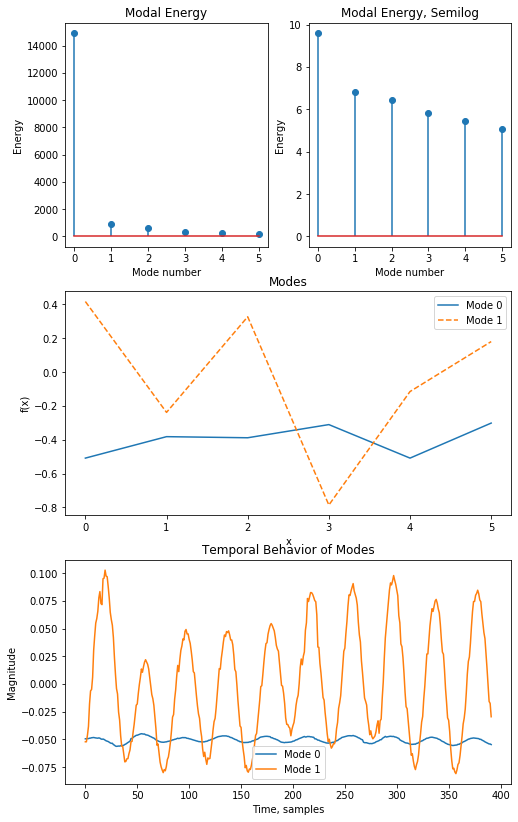
\includegraphics[width=\columnwidth]{kutz4.png}}
	\caption{Kutz Plot, Case 4}
	\label{kutz4}
\end{figure}


\section{Summary and Conclusion}
From these experiments the primary conclusions can be drawn:
\begin{enumerate}
    \item PCA is powerful at decomposing complex, high dimensional data into its constituent parts.
    \item PCA is sensitive to the relative scaling of data, along with the presence of noise.
    \item PCA is sensitive to temporal shifts in data, and unaligned data may produce false modes.
    \item Image tracking is non-trivial and should have plenty of time dedicated to it.
\end{enumerate}

Ultimately, I think I need more time to fully grok the underlying mathematics of SVD/PCA, but I
have no doubt at this point of its wide applicability and power.


\newpage
\clearpage
\newpage
\section{Appendix A: Functions Used}
Commonly used functions, such as plotting, routine mathematical manipulations, and others, are
not included here as they are deemed trivially understood.

\subsection{\code{scipy.io.loadmat}}
Given a path to a *.mat file, load the contents as a dictionary. Includes the header and global
variables that may be included.

\subsection{\code{cv2.cvtColor}}
Converts an image or video to a new color representation, such as RGB, BGR, or Grayscale.
\subsection{\code{cv2.threshold}}
Given a grayscale image or video and a luminance threshold, apply a thresholding function.
Options include binary, to zero, and others.
\subsection{\code{cv2.imshow}}
Show an image using CV2.
\subsection{\code{cv2.selectROI}}
Assuming an image is displayed, allow the user to select a bounding box "region of interest".
\subsection{\code{cv2.TrackerCSRT\_create}}
Create a CSRT tracker. Must be initialzed with a bounding shape and initial frame.
\subsection{\code{cv2.rectangle}}
Draw a rectangle on the active frame with the given corner coordinates, color specification,
and line thickness.
\subsection{\code{cv2.waitKey}}
Waits the given time in milliseconds. If a key is pressed, its value is returned. Used for checking
for early quits ("q" key, here).
\subsection{\code{cv2.destroyAllWindows}}
Method to assert the dominance of *nix systems over weak, MSDOS systems. Kidding, really its an
active method to remove all open windows managed by OpenCV.

\subsection{\code{numpy.load}}
Loads a \code{*.npy} file. Conversions were done on the original \code{*.mat} files to make them
easier to import.
\subsection{\code{numpy.squeeze}}
Given an \code{ndarray} with any axes of size 1, return a copy of the data with the redundant
axes removed. E.g., a (3,1) matrix will become (3,).
\subsection{\code{numpy.stack}}
Given a sequence of arrays in tuple form, join them along a given axis. Used to combine the
individual observations into a data matrix.
\subsection{\code{numpy.linalg.svd}}
Compute the Singular Value Decomposition of the input matrix, and returns the $\myMatrix{U}$,
$\myMatrix{\Sigma}$, and $\myMatrix{V}^{*}$ matrices.

\newpage
\clearpage
\newpage
\section{Appendix B: Python Code}
See my \href{https://github.com/eric-silk/AMATH582_HW3}{Github} for the full repository, including this source code for this IEEE template \LaTeX document. Code is also attached at the end of this report.


\end{document}
